\documentclass[a4paper, 12pt]{article}
\usepackage{fullpage}
\usepackage[german]{babel}
\usepackage{graphicx}
\renewcommand{\figurename}{Schema}
\renewcommand{\tablename}{Tabelle}

\begin{document}

		% Titel
	\title{Praktikumsbericht\\Physkalisches Paktikum\\Linsen und Augenmodell O1}
	\author{von:\\Janosch Ehlers, André Mannweiler\\Gruppe: C2\\\\Tutor: Gian-Luca Woynowski}
	\date{Datum der Versuchsdurchführung:\\ 27.06.2019}
	\maketitle
	\thispagestyle{empty}
\newpage
	\clearpage
	\pagenumbering{arabic}	
\section{Versuchsziel}
	Der Versuch“ Dünne Linsen und Augenmodel“ besteht aus 2 Teilen. In Teil 1 werden die Brennweiten von dünnen Streu- und Sammellinsen durch das Bessel-Verfahren und die Autokollimation bestimmt. In Teil 2 wird das menschliche Auge nachgebildet und mit einer variablen Linse untersucht.

\subsection{Theoretischer Hintergrund}
\subsubsection{Teil 1}
	Methoden der Brennweitenbestimmung
Alle hier genannten Gleichungen gelten für dünne Linsen, die sich dadurch auszeichnen, dass ihre Dicke im Vergleich zu den Krümmungsradien ihrer Oberflächen klein ist. Außerdem besitzen dünne Linsen auf beiden Seiten dieselbe Brennweite. Um die Brennweite einer Linse $f$ über die Gegenstandsweite $a$ und die Bildweite $b$ zu berechnen gilt Gleichung \ref{G_a+b}. Die Gesamtbrennweite $f\textsubscript{ges}$ einer Linse lässt sich über die Addition der beiden einzelnen Brennweiten $f\textsubscript{1}$ und $f\textsubscript{2}$ nach Gleichung \ref{G_f-summe} errechnen. Wenn zwischen Linsen in einem Linsensystem ein Abstand gemessen werden kann, gilt Gleichung \ref{G_mitc}.
	\begin{eqnarray}
	\frac{1}{f}=\frac{1}{a}+\frac{1}{b} \label{G_a+b}\\
	\frac{1}{f_\textsubscript{ges}}=\frac{1}{f\textsubscript{1}}+\frac{1}{f\textsubscript{2}} \label{G_f-summe}\\
	\frac{1}{f\textsubscript{ges}}=\frac{1}{f\textsubscript{1}}+\frac{1}{f\textsubscript{2}}-\frac{c}{f\textsubscript{1}f\textsubscript{2}} 	\label{G_mitc}
	\end{eqnarray}
Zur Messung einer Brennweite sind zwei Verfahren gebräuchlich. Das Besselverfahren und das Autokolimationsverfahren. Für das Besserlverfahren muss $d>4f$ gegeben sein. Hierbei können zwei Linseneinstellungen zwischen Bildebene und Gegenstand gewählt werden,um das Bild scharf auf einem Projektionsschirm darzustellen. Hierbei steht der Abstand $e$ zwischen beiden Linseneinstellungen nach Gleichung \ref{G_1.2_linear-zusammenhang} in einem Linearen Zusammenhang mit der Brennweite der Linse. Das Autokollimationsverfahren benutzt einen gänzlich anderen Ansatz. Hier wird der Schirm durch ein Spiegel ausgetauscht. Die Bildebene ist nun in der Gegenstandsebene. Grundlage dafür ist die Prämisse, dass die Brennweite einer Linse auf beiden Seiten gleich ist.
 %Bild Besselverfahren und Autokollimationsverfahren.

\subsubsection{Teil 2}
	Hier wird versucht ein menschliches Auge nachzustellen. Das menschliche Auge benutzt eine variable Linse um zu fokussieren. Dabei wird die Brennweite der Linse variiert um auf Gegenstandsweitenänderungen zu reagieren.
		
\subsection{Versuchsaufbau}
\subsubsection{Besselverfahren}
	Um die Brennweite einer Sammellinse mithilfe des Bessel-Verfahren zu bestimmen, wird ein Gegenstand (Ampelmännchen) vor die Lampe platziert und in einer definierten Entfernung das Licht auf einen Schirm projiziert. Es wird versucht ein möglichst scharfes Bild einzustellen, indem man die Linse so lange bewegt bis dies der Fall ist. Für jeden Abstand gibt es genau zwei Positionen bei dem die Linse ein scharfes Bild erzeugt. Die Linse ist auf einem Verschiebereiter befestigt, an dem der Abstand genau gemessen werden kann. Zum Verbessern der Auflösung kann zusätzlich eine Blende zwischen Lampe und Blende platziert werden. Die Brennweite einer Zerstreuungslinse wird bestimmt, indem man diese mit der zuvor gemessenen Zerstreuungslinse kombiniert. Durch die Messung des Gesamtsystems beider Linsen und den Werten der vorherigen Messung kann man Werte der Zerstreuungslinse errechnen. Die beiden Linsen werden zusammen in der Linsenhalterung platziert. Danach wird bereits wie beim Bessel-verfahren der Sammellinse vorgegangen.

\subsubsection{Autokollimationsverfahren}
	Die Brennweiten der Sammellinsen und der Zerstreuungslinse soll mithilfe des Autokollimationsverfahrens überprüft werden. Dazu wird der Schirm durch einen Spiegel ersetzt und wie oben beschrieben, die Bildebene in der Gegenstandsebene abgebildet. Es wird versucht ein möglich scharfes Bild zu erhalten, indem man das Spiegel-Linsensystem verschiebt. Dies macht man für jede Linse zweimal, in dem man sie bei der zweiten Messung um ca. 180$^\circ$ verschiebt und aus der resultierenden abstandsdifferenz den Mittelwert bildet. Dadurch wird der Fehler minimiert, der sich aus dem Ablesefehler und einem Aufbaufehler bei dem aufbau der Linse ergibt.

\subsubsection{Augenmodell}
Hier wird mit einer variablen Linse gearbeitet. Durch Zugabe von Flüssigkeit in die Linse kann diese gedehnt werden. Die Krümmung und Brechkraft dieser wird dadurch variiert. Die Anordnung der Elemente am Reiter bleibt die gleiche wie beim Bessel-Verfahren. Die Irisblende wird jedoch zusätzlich verwendet um das Licht zu achsennahe Strahlen zu bündeln. Für die Autokollimation wird die Linse mit 50ml leicht saurem Wasser befüllt und solange verschoben bis man ein scharfes Bild erhält. Iterrativ wird nun das Füllvolumen um 10\ ml erhöht. Da die Brennweite der Linse reziprokporortional zu ihrem Füllvolumen ist, kann damit ein Proportionalitätsfaktor ausgerechnet werden. Dieser wird im späteren verlauf wichtg. Zusätzlich wird ein weitsichtiges Auge und ein weitsichtiges mit Sehhilfe simuliert und die Brennweiten mithilfe des Bessel-Verfahrens bestimmt und disskutiert. 

%	\begin{table}
%		\centering
%		\begin{tabular}{l||c|c|c}
%			Aufgabe &  & f & $\Delta$f\\\hline
%			1.2 &  & 144,274452250879 & 3,99846815063194\\\hline
%			1.3 &  & 128,414323492827 & 45,5464923370223\\\hline
%			1.4 & Sammel 7,5 \& Streulinse & 92 & 0,5\\\hline
%			 & Sammel 7,5 1 & 73,25 & 0,5\\\hline
%			 & Sammel 15 1 & 93,5 & 0,5\\\hline
%			 & Sammel 15 2 & 95,75 & 0,5\\\hline
%			\hline
%			 &  & K & $\Delta$K\\\hline
%			2.1 &  & 12758,3333333333 & 78,0115732154887\\
%		\end{tabular}
%		\caption{Messergebnisse}			
%	\end{table}

\section{Auswertung}
\subsection{Versuch 1.1}
	Die Brennweiten der zuverfügung stehenden Sammellinsen ergab, dass Zwei Linsen eine ungefähre Brennweite von 15\ cm die dritte Sammellinse hat eine ungefähre Brennweite von 7,5\ cm.\\

\subsection{Versuch 1.2}
	Die Bestimmung der Brennweite einer Sammellinse, dessen Brennweite im vorhinein auf $\approx 15$\ cm geschätzt wurde ergab nach Gleichung \ref{G_1.2_linear-zusammenhang} ein Wert von 144,27\ mm. Der Fehler errechnet sich nach Gleichung \ref{G_1.2_Fehler1}. Endgültig errechnet sich ein Fehler von 4\ mm. Ein Diagramm, in welchem $\frac{e^2}{d}$ über $d$ inklusive der Ausgleichsgeraden ist in Schema \ref{Abb1.2} Abbgebildet.
	\begin{eqnarray}
		\frac{e^2}{d}&=&d-4\cdot f \label{G_1.2_linear-zusammenhang}\\
		\Delta f&=&f^{-2}\cdot\sqrt{(\Delta a\cdot a^{-2})^2+(\Delta b\cdot b^{-2})^2} \label{G_1.2_Fehler}\\
		f&\sim &\frac{1}{V}\label{G_Prop_K}
	\end{eqnarray}
\subsection{Versuch 1.3}
Die Brennweite der Zersteuungslinse wurde über umstellen der Gleichung \ref{G_f-summe} nach $f\textsubscript{1}$ berechnet. Da die Gesamtbrennweite des Linsensystems über das gleiche Verfahren ermittelt werden kann wie in Versuch 1.2 beschreiben und die Brennweite der Sammellinse theoretisch bekannt ist, kann über umstellen der O.g. Gleichung die Brennweite bestimmt werden. Ein Diagramm inder die Experimentellen Werte inklusive einer Ausgleichsgeraden aufgelistet werden ist in Schema \ref{1.3} zusehen. Der Fehler sich ebenfalls nach \ref{G_1.2_Fehler} auf $\pm$45,55\ mm. Die Brennweite der Streulinse ist also $f=(128,41\pm45,55)\ mm$ Zur überprüfung durch das Autokollimationsverfahren ist die Gegenstandweite gleich der Brennweite. Ebenfalls beschränken sich die Fehler auf die Ablesefehler auf der Reiterskaler. Es ergeben sich also folgende Werte:\\

	\begin{center}
	\begin{tabular}{c|cc}
 & $f$ & $\Delta f$\\
 \hline
		Sammel 7,5 \& Streulinse &92&0,5\\
		Sammel 7,5 &73,25&0,5\\
		Sammel 15 1&93,5&0,5\\
		Sammel 15 2&95,75&0,5\\
	\end{tabular}
	\end{center}
Auch, wenn hier die errechneten Fehler ziemlich gering sind, weichen die Errechneten Werte doch Stark von den in 1.2 und 1.3 ab. Grund ist sehr Wahrscheinlich die schlechte Bestimmung des Fokuspunkts auf der sehr hellen Gegenstandsebene.

	\begin{eqnarray}
		K&=&f\cdot V\label{G_2.1_K}\\
		\Delta K&=&\sqrt{(\Delta f\cdot V)^2+(\Delta V\cdot f)^2}\label{G_2.1_K-Fehler}
	\end{eqnarray}
Der in 1.2.3 genannte Proportionalitätsfaktor wird nun über Gleichung \ref{G_2.1_K} errechnet. Da hier immernoch ein Autokollimationsverfahren verwendet wird kann die Brennweite direkt abgelesen werden. Der Fehler errechnet sich nun nach Gleichung \ref{G_2.1_K-Fehler}. Wir erhalten ein$ $K von $K=(12758,33\pm 78,01)\ mm\cdot ml$ \\ Dieser Proportionalitätsfaktor ist nun nützlich um in Versuch 2.4 die Brennweite der variablen Linse zu ermitteln. Die Diagramme in der $f$ über $a$ für das normalsichtige Auge, das weitsichtige Auge und dem weitsichtigen Augen mit Sehhilfe aufgetragen ist. In Abbildung \ref{Abb2.2} und \ref{Abb2.3} zusehen.
Die Brennweiten des Weitsichtigen Auges mit Sehhilfe ist in der nachfolgenden Liste zusehen:
\begin{enumerate}
\item $(318,96\pm 8,21)\ $mm
\item $(255,17\pm 5,34)\ $mm
\item $(227,83\pm 4,3)\ $mm
\item $(212,64\pm 3,77)\ $mm
\item $(199,35\pm 3,34)\ $mm
\item $(187,62\pm 2,99)\ $mm
\item $(163,57\pm 2,32)\ $mm
\item $(135,73\pm 1,67)\ $mm
\end{enumerate}

\newpage
\begin{figure}
\centering
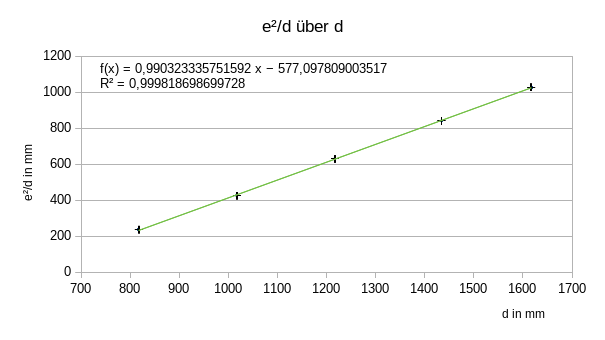
\includegraphics[scale=0.7]{12.png}
\caption{Brennweite Sammellinse 15}
\label{Abb1.2}
\end{figure}

\begin{figure}
\centering
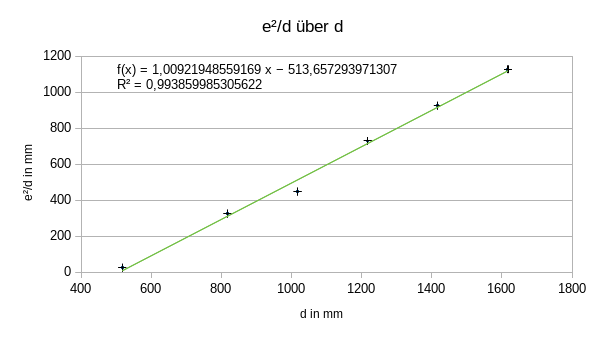
\includegraphics[scale=0.7]{13.png}
\caption{Brennweite Streulinse}
\label{Abb1.3}
\end{figure}

\begin{figure}
\centering
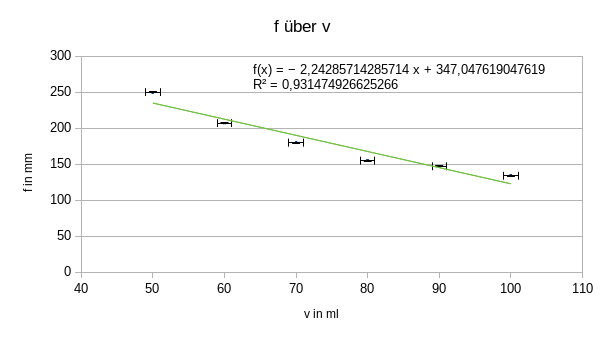
\includegraphics[scale=0.7]{21.png}
\caption{Proportionalitätsfaktor}
\label{Abb2.1}
\end{figure}

\begin{figure}
\centering
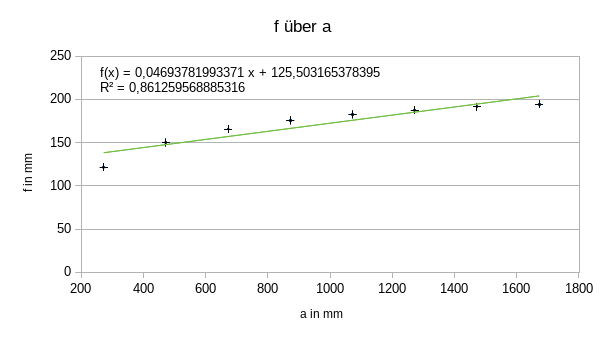
\includegraphics[scale=0.7]{22.png}
\caption{Normalsichtiges Auge}
\label{Abb2.2}
\end{figure}

\begin{figure}
\centering
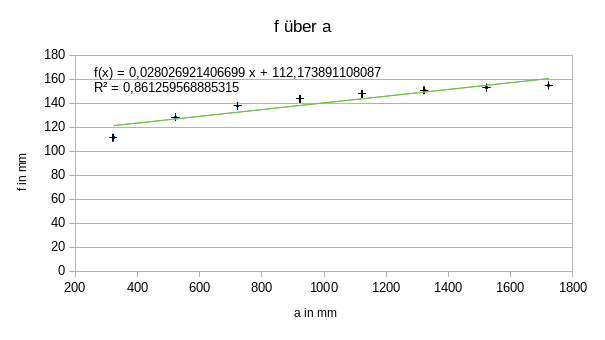
\includegraphics[scale=0.7]{23.png}
\caption{Weitsichtiges Auge ohne Sehhilfe}
\label{Abb2.3}
\end{figure}


\end{document}